\section[Definition and Frequencies of Time Series Data]{Definition and Frequencies of Time Series Data\label{ex:DefinitionFrequenciesTimeSeriesData}}

\begin{enumerate}
	\item Briefly define a time series in terms of random variables and stochastic processes.	
	\item Consider data for various time series given in
	\begin{itemize}
		\item \texttt{NorwayGDP.xls}
		\item \texttt{NorwayInterestRate3m.xls} 
		\item \texttt{NorwayInterestRate10yrs.xls}
		\item \texttt{NorwayOSEBXGR.csv}
		\item \texttt{NorwayPopulation.xls}
		\item \texttt{NorwayRealHousePrices.xlsx}
		\item \texttt{NorwayUnemploymentRate.xls}
	\end{itemize}
	Open the individual files and make note of the structure and source of the data.
	Import the data and replicate figure \ref{fig:NorwayData}.
	   \begin{figure}[htbp]
		\centering
		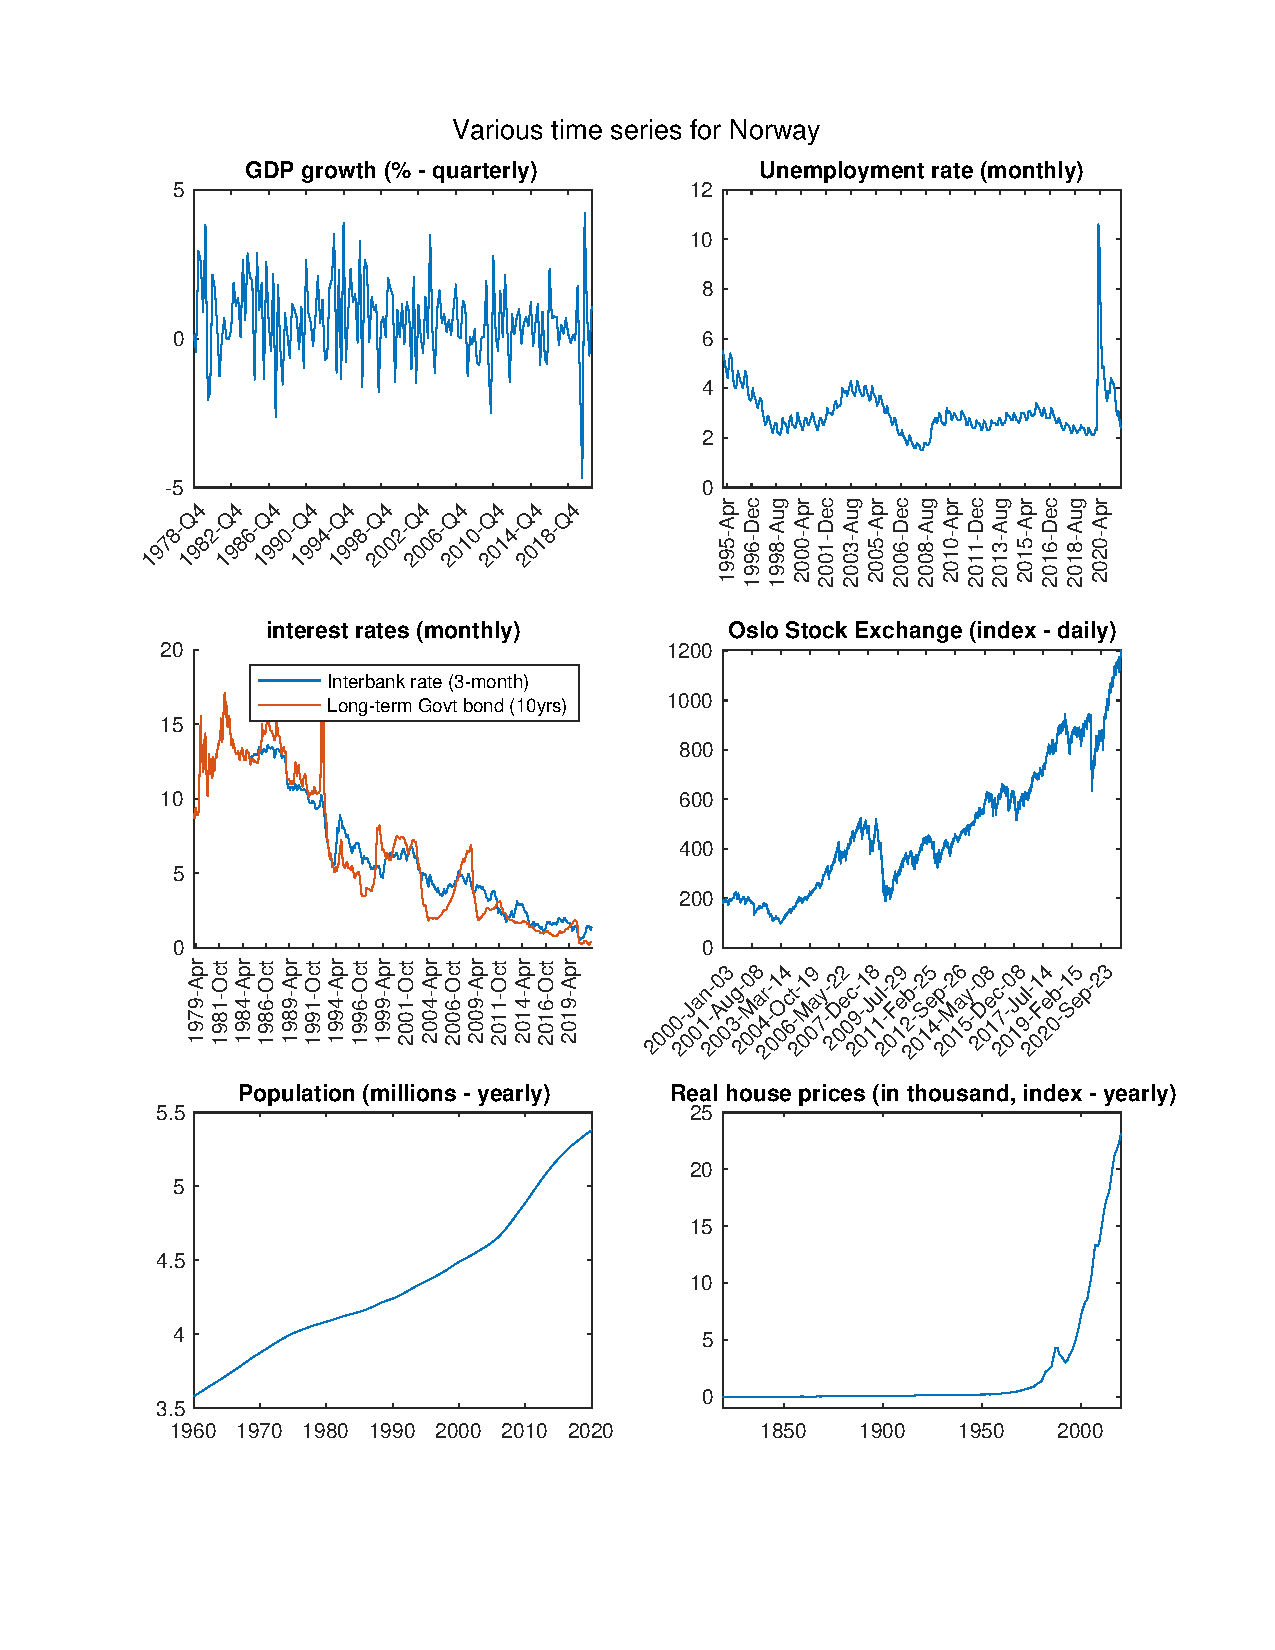
\includegraphics[width=\linewidth]{plots/NorwayDataOverviewMatlab.pdf}
		\caption{Various Time Series For Norway}
		\label{fig:NorwayData}
		\end{figure}
   \item What are the data frequencies for each time series?
   For what kind of economic analysis would you use these frequencies?
   \item What are the sample sizes?
   From an economic and/or statistical point of view, is it always better to have a larger sample size?
   \item Roughly speaking, a time series consists of four components: a trend, a cycle, a season, and noise.
   To what extent do you find these features in figure \ref{fig:NorwayData}?
   \item Consider the plots in figure \ref{fig:NorwayData} jointly.
   What are possible macroeconomic issues that could be analyzed?
   \item How do you aggregate time series of stock variables (like capital or debt) and of flow variables (like GDP)?
   For example, if you have monthly data, how do you get a quarterly time series?
\end{enumerate}

\paragraph{Readings}
\begin{itemize}
   \item \textcite[Ch.1, Ch.2]{Bjornland.Thorsrud_2015_AppliedTimeSeries}
\end{itemize}

\begin{solution}\textbf{Solution to \nameref{ex:DefinitionFrequenciesTimeSeriesData}}
\ifDisplaySolutions
\begin{enumerate}
\item A time series is a collection of observations \(Y_t\) indexed by the date of each observation \(t\).
For simplicity often one denotes \(t=0,1,2,\ldots ,T\),
  then \( {\{Y_t\}}_0^T = \{Y_0,Y_1,Y_2,\ldots ,Y_T\} \) is a sequence of random variables ordered in time
  (each \(Y_t\) is a random variable), which we call a stochastic process.
Sometimes we rely on the concept of an infinite sample and consider \( {\{Y_t\}}_{t=-\infty}^\infty \) or simply \( \{Y_t\} \).
A stochastic process can have many outcomes, due to its randomness,
  and a single outcome of a stochastic process is called a sample function or realization.
A time series model assigns a joint probability distribution to the stochastic process.
\item Most of the files are downloaded from FRED except \texttt{NorwayOSEBXGR.csv} which is downloaded from Euronext and \texttt{NorwayRealHousePrices.xlsx} from the Norges Bank in October 2021.
\lstinputlisting[style=Matlab-editor,basicstyle=\mlttfamily,title=\lstname]{progs/matlab/definitionFrequenciesTimeSeriesData.m}
\item Wide range of frequencies:
\begin{itemize}
    \item Daily data: Oslo Stock Exchange
    \item Monthly data: Interest rates, unemployment rate
    \item Quarterly data: GDP growth
    \item Yearly data: population and real house price index
\end{itemize}
For business cycle analysis one usually focuses on monthly or quarterly data;
  for understanding stock returns we consider daily or monthly data;
  for long-run growth and wealth of nations considerations yearly data might be sufficient.
\item Sample sizes vary considerably. While quarterly data of GDP growth covers a much shorter sample than yearly house prices series,
  the number of observations are not that different.
Higher frequencies typically mean more observations.
On the one hand, many results in statistics and econometrics depend on having many observations, so the more the better.
On the other hand consider for example the stock market index.
We have nearly 300 business day observations every year.
However, information in all these daily data does not say much about, say, the overall state of the economy.
We rather have several periods:
  prior to mid 2003 when stock index hovered around 200,
  run-up to the financial crisis period from mid-2007 to mid-2008,
  the sharp fall during the financial crisis,
  the continuous recovery afterwards
  and then Covid.
From a macroeconomic perspective we rather have a couple of \enquote{informative} periods, evident in monthly or quarterly data,
  all other daily observations are more or less just noise.
So it is not always better to have a larger sample size if is uninformative.
\item For the different figures
\begin{itemize}
    \item GDP growth: no trend, pronounced cyclical patterns (business cycles), no seasonality (data is seasonally adjusted), much noise
    \item Unemployment rate: no trend, pronounced cyclical patterns (business cycles), seasonality evident (data is not seasonally adjusted), some noise
    \item interest rates: downward (linear) trend, pronounced cyclical patterns in long-term yields, less so in short-term, no seasonality, moderate noise
    \item Oslo stock Exchange: upward (piecewise-linear) trend, cyclical patterns, no seasonality, moderate noise
    \item Population: upward (linear) trend, no cyclical patterns, no seasonality, no noise
    \item Real house prices: upward (exponential) trend, no cyclical patterns, no seasonality, no noise
\end{itemize}
\item We could analysis for instance:
    \begin{itemize}
        \item While financial crisis is clearly visible in the stock exchange,
          the effect on unemployment rate or real house prices is hard to detect.
        Real income, job opportunities and consumer confidence remained high. Why?
        \begin{itemize} 
            \item Maybe monetary policy influenced the behavior of the unemployment rate as Figure c indicates expansionary monetary policy.
            \item Or Norwegian oil sector is highly productive (makes up 25\% of GDP) so is this the reason why the financial crisis was cushioned?
        \end{itemize}
        \item Are house prices in line with their fundamentals? Is there a bubble?
    \end{itemize}
\item Aggregation of higher frequencies to lower frequencies is straightforward;
  that is, for stock variables (such as capital or debt) we simply take the value observed, i.e.\
  \(k_t^{Q1} = k_t^{m3}\),
  whereas for flow variables (such as GDP) we can take the mean: \(y_t^{Q1} = 1/3 (y_t^{m1}+y_t^{m2}+y_t^{m3})\).
Disaggregation is much more difficult and we need to use tools like interpolation or spline functions etc.\
  \(\rightarrow \) not straightforward!
\end{enumerate}
\fi
\newpage
\end{solution}